\documentclass[a4paper, 11pt]{article}
\usepackage{comment} 
\usepackage{fullpage}
\usepackage{amsmath} 
\usepackage{amssymb} 
\usepackage{mathtools}
\usepackage{fontspec}
\defaultfontfeatures{Ligatures=TeX}
\usepackage{xfrac}
\usepackage{icomma}
\usepackage[section,below]{placeins}
\usepackage[labelfont=bf,font=small,width=0.9\textwidth]{caption}
\usepackage{subcaption}
\usepackage{graphicx}
\usepackage{grffile}
\usepackage{float}
\floatplacement{figure}{htbp}
\floatplacement{table}{htbp}
\usepackage{booktabs}
\usepackage{hyperref}
\usepackage[ngerman]{babel}
\usepackage{pdfpages}
\begin{document}
\noindent
%\centerline{\small{\textsc{Technische Universität Dortmund}}} \\
\large{\textbf{6. Übungsblatt zur Vorlesung \hfill WS 2017/2018 \\
Statistische Methoden der Datenanalyse \hfill Prof. W. Rhode}} \\
Annika Burkowitz, Sebastian Bange, Alexander Harnisch \\
\noindent\makebox[\linewidth]{\rule{\textwidth}{0.4pt}}

\section*{Aufgabe 19}
\subsection*{a)}
Wenn eine ungewichtete Norm wie die euklidische Norm für die Abstandsberechnung
verwendet wird und sich die Attribute in der Größenordnung unterscheiden, dann
haben die größeren Attribute in der Abstandsberechnung ein deutlich höhere
Gewicht. Es ist praktisch nur noch der Abstand des größten Attributs relevant,
der Rest spielt keine Rolle mehr. Bspw. Abstand der zwei Punkte $a = (1, 10000,
5)^{\textup{T}}$ und $b = (3, 10232, 9)^{\textup{T}}$:
\begin{equation}
    \sqrt{(a - b)^2} \approx b_2 - a_2 = 232\,.
\end{equation}

\subsection*{b)}
Der $k$-NN-Algorithmus wird als \textit{lazy learner} bezeichnet, weil
praktisch der gesamte Rechenaufwand in die Anwendungs-Phase gelegt wird. Anders
als bspw. beim Random Forest Verfahren, bei dem in der Lernphase
rechenaufwendig Bäume erstellt werden, die sich in der Anwendungsphase mit
relativ geringem Rechenaufwand auswerten lassen.

\subsection*{d)}
\begin{center}
    \begin{tabular}{cc}
        Reinheit: & 0,8340\\
        Effizienz: & 0,9644\\
        Genauigkeit: & 0,9242\\
        Signifikanz: & 66,76\\
    \end{tabular}
\end{center}

\subsection*{e)}
\begin{center}
    \begin{tabular}{cc}
        Reinheit: & 0,8712\\
        Effizienz: & 0,9813\\
        Genauigkeit: & 0,9454\\
        Signifikanz: & 65,03\\
    \end{tabular}
\end{center}

\subsection*{f)}
\begin{center}
    \begin{tabular}{cc}
        Reinheit: & 0,8590\\
        Effizienz: & 0,9859\\
        Genauigkeit: & 0,9414\\
        Signifikanz: & 66,26\\
    \end{tabular}
\end{center}

\section*{Aufgabe 20}
\subsection*{e, f)}
\FloatBarrier
\begin{figure}
    \centering
    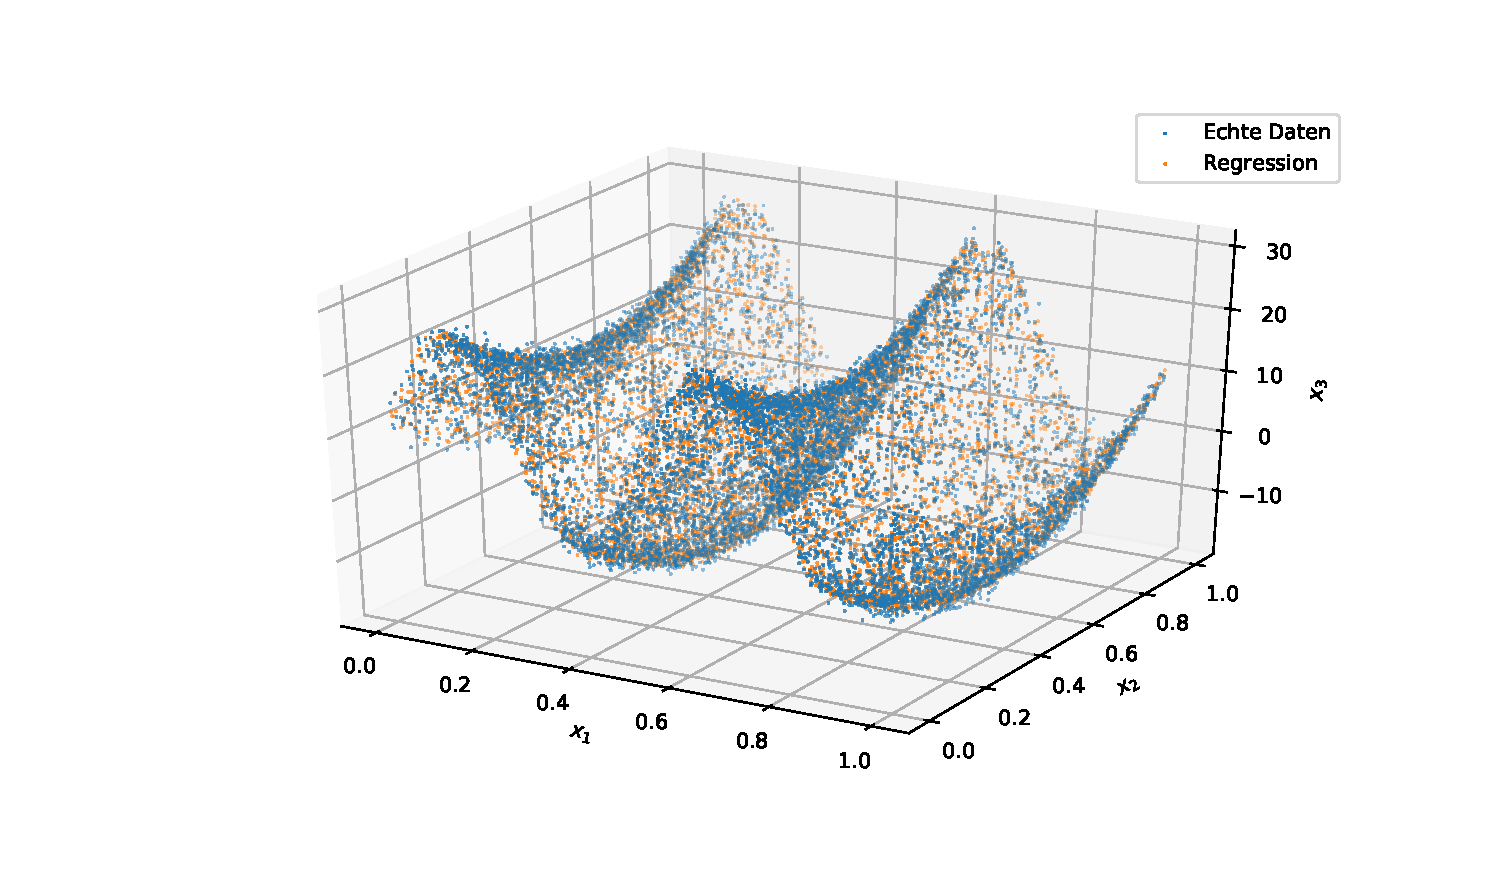
\includegraphics[width=\textwidth]{../A20/A20_3D_e.pdf}
    \caption{3D-Plot, mit $x_1, x_2\in\{0, 1\}$.}
\end{figure}

\begin{figure}
    \centering
    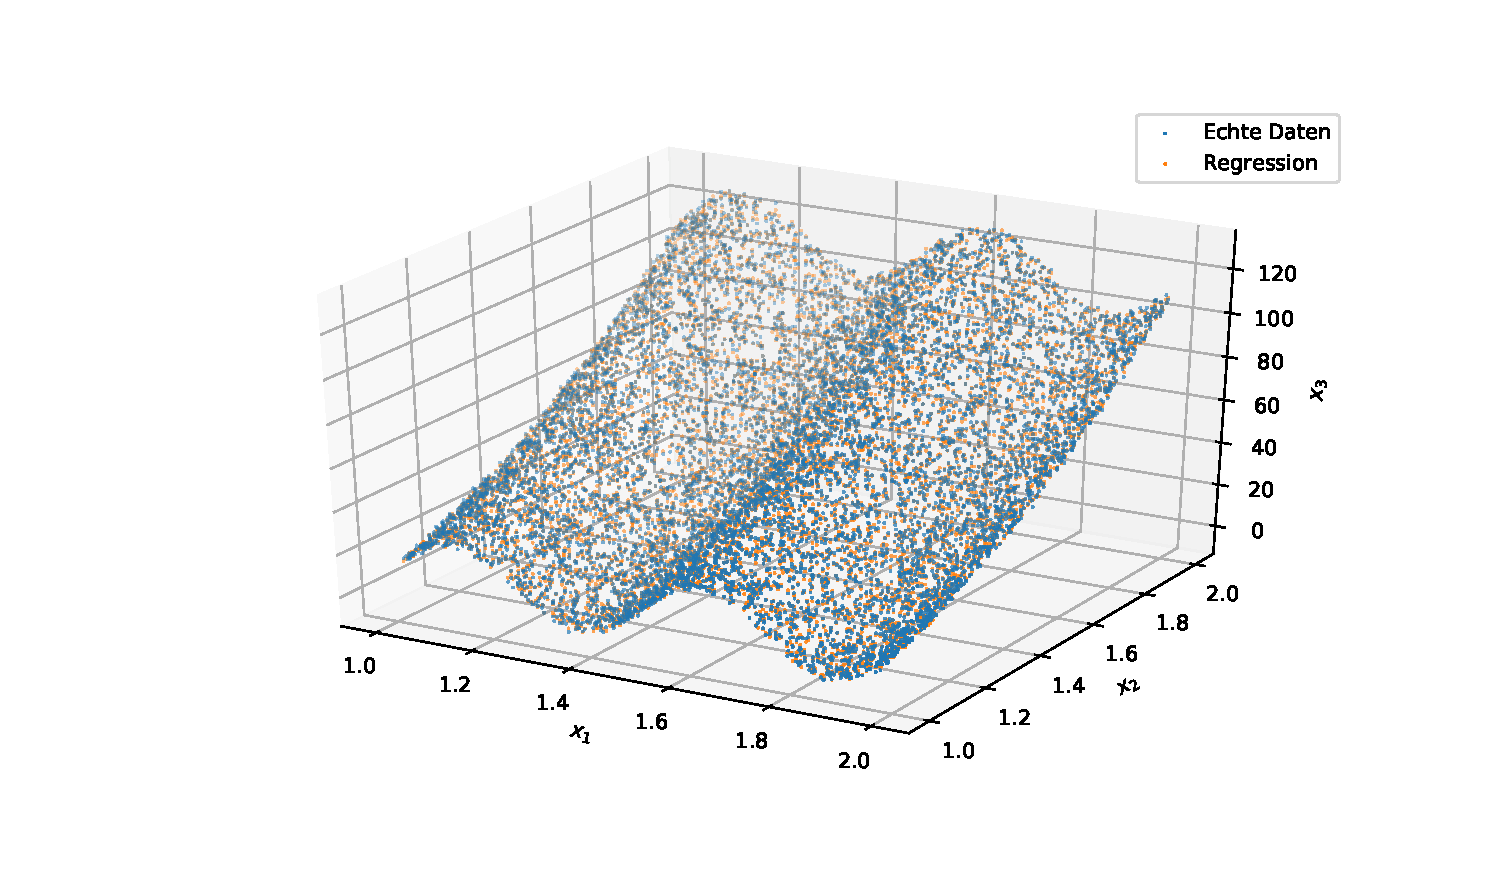
\includegraphics[width=\textwidth]{../A20/A20_3D_f.pdf}
    \caption{3D-Plot, mit $x_1, x_2\in\{1, 2\}$.}
\end{figure}

\begin{figure}
    \centering
    \includegraphics[width=\textwidth]{../A20/A20_x1_x3_e.pdf}
    \caption{Projektion in die $x_1, x_3$-Ebene, mit $x_1, x_2\in\{0, 1\}$.}
\end{figure}

\begin{figure}
    \centering
    \includegraphics[width=\textwidth]{../A20/A20_x1_x3_f.pdf}
    \caption{Projektion in die $x_1, x_3$-Ebene, mit $x_1, x_2\in\{1, 2\}$.}
\end{figure}

\begin{figure}
    \centering
    \includegraphics[width=\textwidth]{../A20/A20_x2_x3_e.pdf}
    \caption{Projektion in die $x_2, x_3$-Ebene, mit $x_1, x_2\in\{0, 1\}$.}
\end{figure}

\begin{figure}
    \centering
    \includegraphics[width=\textwidth]{../A20/A20_x2_x3_f.pdf}
    \caption{Projektion in die $x_2, x_3$-Ebene, mit $x_1, x_2\in\{1, 2\}$.}
\end{figure}

\begin{figure}
    \centering
    \includegraphics[width=\textwidth]{../A20/A20_x3_x3_e.pdf}
    \caption{Geschätzter $x_3$-Wert gegen den echten $x_3$-Wert (optimal ist eine Gerade mit Steigung 1), mit $x_1, x_2\in\{0, 1\}$.}
\end{figure}

\begin{figure}
    \centering
    \includegraphics[width=\textwidth]{../A20/A20_x3_x3_f.pdf}
    \caption{Geschätzter $x_3$-Wert gegen den echten $x_3$-Wert (optimal ist eine Gerade mit Steigung 1), mit $x_1, x_2\in\{1, 2\}$.}
\end{figure}

\begin{center}
    \begin{tabular}{cc}
        MSE, $x_1, x_2\in\{0, 1\}$: & 1,245 \\
        MSE, $x_1, x_2\in\{1, 2\}$: & 1,404\\
    \end{tabular}
\end{center}

\includepdf{../A21/Rechnung.pdf}

\section*{Aufgabe 21}
\subsection*{c)}
\begin{figure}
    \centering
    \includegraphics[width=\textwidth]{../A21/Temperatur.pdf}
    \caption{Untersuchung des Attributes "Temperatur".}
\end{figure}
\begin{figure}
    \centering
    \includegraphics[width=\textwidth]{../A21/Wettervorhersage.pdf}
    \caption{Untersuchung des Attributes "Wettervorhersage".}
\end{figure}
\begin{figure}
    \centering
    \includegraphics[width=\textwidth]{../A21/Luftfeuchtigkeit.pdf}
    \caption{Untersuchung des Attributes "Luftfeuchtigkeit".}
\end{figure}
\FloatBarrier

\subsection*{d)}
Da bei der Temperatur der höchste Informationsgewinn vorliegt, ist das das beste Attribut zum Trennen der Daten.

\end{document}
